% =====================================================================
%  Chapitre 4 -- Entraînement, régularisation et transfert
%  Partie a : entraînement, learning rate, optimiseurs, courbes
% =====================================================================
\section{Chapitre 4 --- Entraînement, régularisation, transfert}

\chapterslide{Chapitre 4}{Entraînement, régularisation et transfert}%
{5 h --- entraîner un CNN, lutter contre le surapprentissage, réutiliser un modèle}%
{\textbf{Objectifs.} Mettre en place la boucle d'entraînement (époques, lots,
itérations) ; choisir un pas d'apprentissage et un optimiseur (SGD, momentum, Adam) ;
lire des courbes d'apprentissage ; connaître les techniques de régularisation
(dropout, batch normalization, weight decay, early stopping) ; augmenter les
données et faire du transfert learning.}

\begin{frame}{Plan du chapitre}
\begin{columns}[t]
\begin{column}{0.48\textwidth}
\begin{kbox}[Les quatre temps de ce chapitre]
\begin{enumerate}
  \item La boucle d'entraînement : époques, lots, itérations.
  \item Le pas d'apprentissage et les optimiseurs.
  \item Lire les courbes : sous- et surapprentissage.
  \item Régulariser, augmenter, transférer.
\end{enumerate}
\end{kbox}
\end{column}
\begin{column}{0.48\textwidth}
\begin{ebox}[Ce que vous saurez faire]
\begin{itemize}
  \item Écrire une boucle d'entraînement PyTorch complète.
  \item Diagnostiquer un modèle à partir de ses courbes.
  \item Choisir un optimiseur et son pas d'apprentissage.
  \item Mettre en place dropout, augmentation et transfert.
\end{itemize}
\end{ebox}
\end{column}
\end{columns}
\vspace{1mm}
\begin{wbox}[Le fil rouge de ce chapitre]
Un CNN mal entraîné ne vaut rien : une architecture savante et un entraînement
négligé donnent un mauvais modèle. Tout le chapitre porte sur \emph{comment}
apprendre les poids, et sur les garde-fous qui empêchent le réseau d'apprendre
« par cœur » au lieu d'apprendre le motif.
\end{wbox}
\end{frame}

\begin{frame}{Entraîner, c'est répéter trois gestes}
\begin{columns}[t]
\begin{column}{0.54\textwidth}
\begin{itemize}
  \item \textbf{Prédire} : on présente un lot au réseau, il produit une sortie.
  \item \textbf{Mesurer l'erreur} : une fonction de coût compare la sortie à
  l'étiquette attendue.
  \item \textbf{Corriger} : on calcule le gradient de l'erreur par rétropropagation,
  puis on déplace les poids dans le sens opposé.
\end{itemize}
\begin{kbox}[Un seul mot d'ordre : minimiser le coût]
L'entraînement est un problème d'optimisation. Le réseau ne « comprend » rien :
il descend une pente dans un espace de plusieurs millions de dimensions.
\end{kbox}
\end{column}
\begin{column}{0.42\textwidth}
\begin{ebox}[La boucle, vue de loin]
\begin{center}
\small
prédire $\to$ coût $\to$ gradient $\to$ mise à jour

\medskip
\emph{et on recommence}

\medskip
milliers de fois
\end{center}
\end{ebox}
\begin{wbox}[Ce qui peut mal tourner]
Trop lent, instable, bloqué dans un plateau, ou au contraire
« apprentissage par cœur ». Les réglages de cette boucle décident de tout.
\end{wbox}
\end{column}
\end{columns}
\end{frame}

\begin{frame}{Époque, lot, itération : trois mots à ne pas confondre}
\begin{columns}[t]
\begin{column}{0.50\textwidth}
\begin{itemize}
  \item Une \textbf{époque} (\emph{epoch}) : un passage complet sur tout le jeu
  d'entraînement.
  \item Un \textbf{lot} (\emph{batch}) : un sous-ensemble d'exemples traité
  d'un coup.
  \item Une \textbf{itération} : le traitement d'\emph{un} lot, suivi d'\emph{une}
  mise à jour des poids.
\end{itemize}
\end{column}
\begin{column}{0.46\textwidth}
\begin{kbox}[La relation à retenir]
\[
\text{itérations par époque} = \left\lceil \frac{N}{B} \right\rceil
\]
$N$ : nombre d'exemples ; $B$ : taille du lot.
\end{kbox}
\begin{ebox}[Exemple chiffré]
$N = 60\,000$ images, $B = 64$ : environ $938$ itérations par époque.
\end{ebox}
\end{column}
\end{columns}
\vspace{1mm}
\begin{wbox}[Taille du lot : le compromis]
Grand lot : gradient plus stable mais mémoire plus lourde. Petit lot : plus de
bruit (parfois bénéfique), mise à jour plus fréquente. La taille du lot change
la \emph{qualité} de chaque pas, pas seulement sa vitesse.
\end{wbox}
\end{frame}

\begin{frame}{L'anatomie d'un pas d'apprentissage}
\begin{columns}[t]
\begin{column}{0.52\textwidth}
\begin{center}
\begin{tikzpicture}[
  node distance=6mm,
  box/.style={draw=byBlue,thick,rounded corners,fill=byBlue!6,align=center,
              inner sep=3pt,font=\scriptsize}]
\node[box] (a) {charger un lot \quad $\mathbf{X}, \mathbf{y}$};
\node[box,below=of a] (b) {passe avant $\to$ prédiction $\hat{\mathbf{y}}$};
\node[box,below=of b] (c) {coût $\mathcal{L}(\hat{\mathbf{y}},\mathbf{y})$};
\node[box,below=of c] (d) {rétropropagation $\to$ gradients};
\node[box,below=of d] (e) {optimiseur $\to$ nouveaux poids};
\draw[-{Latex}] (a)--(b); \draw[-{Latex}] (b)--(c);
\draw[-{Latex}] (c)--(d); \draw[-{Latex}] (d)--(e);
\draw[-{Latex}] (e.west) -- ++(-6mm,0) |- (a.west);
\end{tikzpicture}
\end{center}
\end{column}
\begin{column}{0.44\textwidth}
\begin{itemize}
  \item Les cinq étapes se répètent à chaque itération.
  \item La rétropropagation est \emph{inclus} dans PyTorch : un appel à
  \py{loss.backward()}.
  \item L'optimiseur ne fait qu'appliquer la règle de mise à jour.
\end{itemize}
\begin{kbox}[Le ``pas'' ne se fait pas tout seul]
Sans \py{optimizer.step()}, les gradients sont calculés mais jamais appliqués :
le réseau n'apprend rien. C'est l'erreur la plus fréquente du débutant.
\end{kbox}
\end{column}
\end{columns}
\end{frame}

\begin{frame}{Le pas d'apprentissage : trois régimes}
\begin{columns}[t]
\begin{column}{0.50\textwidth}
\centering
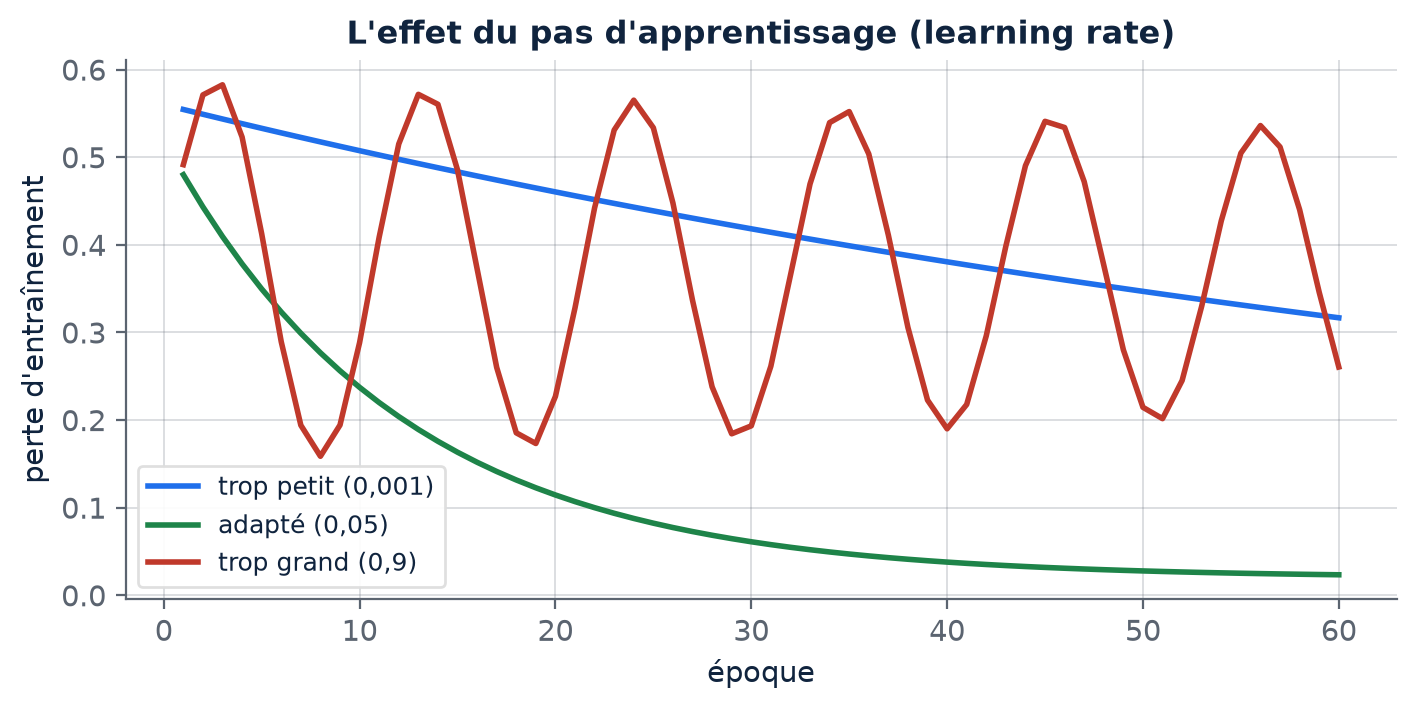
\includegraphics[width=\textwidth]{i06_learning_rate.png}
\end{column}
\begin{column}{0.46\textwidth}
\begin{itemize}
  \item \textbf{Trop petit} ($10^{-3}$, courbe lente) : la descente traîne,
  l'entraînement n'aboutit pas dans le temps imparti.
  \item \textbf{Adapté} (de l'ordre de $5\times10^{-2}$) : la perte chute
  rapidement puis se stabilise.
  \item \textbf{Trop grand} ($9\times10^{-1}$) : la perte oscille, explose ;
  on ne converge pas.
\end{itemize}
\end{column}
\end{columns}
\end{frame}

\begin{frame}{Le pas d'apprentissage : ce qu'il faut en retenir}
\begin{columns}[t]
\begin{column}{0.52\textwidth}
\begin{center}
\begin{tabular}{@{}lll@{}}
\toprule
\textbf{Régime} & \textbf{Pas testé} & \textbf{Comportement} \\
\midrule
Trop petit & $0{,}001$ & lenteur, sous-entraînement \\
Adapté & $0{,}05$ & chute puis stabilisation \\
Trop grand & $0{,}9$ & oscillations, divergence \\
\bottomrule
\end{tabular}
\end{center}
\begin{kbox}[La bonne pratique]
On commence autour de $10^{-3}$, et l'on ajuste : on divise le pas (ou on
utilise un \emph{planificateur}) quand la perte plafonne.
\end{kbox}
\end{column}
\begin{column}{0.46\textwidth}
\begin{wbox}[Ce ne sont pas des vérités absolues]
Les valeurs dépendent du modèle et du jeu de données. Ce qui compte, c'est
l'\emph{allure} de la courbe : elle révèle le régime, pas le chiffre exact.
\end{wbox}
\begin{ebox}[Deux leviers]
\textbf{Planificateurs} (\emph{schedulers}) : réduire le pas par paliers.
\textbf{Cycliques} : faire varier le pas entre deux bornes pour sortir d'un
plateau ou d'un minimum médiocre.
\end{ebox}
\end{column}
\end{columns}
\end{frame}

\begin{frame}{SGD : la règle de base}
\begin{columns}[t]
\begin{column}{0.52\textwidth}
\begin{itemize}
  \item \textbf{Descente de gradient stochastique} : on remplace le gradient
  exact (sur tous les exemples) par son estimation sur un lot.
  \item Mise à jour, pour chaque poids $w$ :
\end{itemize}
\[
w \leftarrow w - \eta \, \nabla_w \mathcal{L}
\]
\begin{itemize}
  \item $\eta$ : le pas d'apprentissage ; $\nabla_w \mathcal{L}$ : le gradient
  estimé sur le lot courant.
\end{itemize}
\begin{kbox}[Simple, mais capricieux]
SGD est la brique de base. Sur une surface en « vallée étroite », il zigzague :
lent dans la direction utile, bruité dans la direction transversale.
\end{kbox}
\end{column}
\begin{column}{0.46\textwidth}
\begin{ebox}[Le bruit : une arme à double tranchant]
Estimer le gradient sur un lot introduit du bruit. Ce bruit aide à ne pas
rester coincé dans un mauvais minimum, mais rend la trajectoire irrégulière.
\end{ebox}
\begin{wbox}[Toujours remettre les gradients à zéro]
PyTorch \emph{accumule} les gradients : oublier \py{optimizer.zero_grad()}
fait s'additionner les gradients de plusieurs itérations.
\end{wbox}
\end{column}
\end{columns}
\end{frame}

\begin{frame}{Momentum : on garde de l'élan}
\begin{columns}[t]
\begin{column}{0.50\textwidth}
\begin{itemize}
  \item Idée : au lieu de suivre uniquement le gradient courant, on le lisse
  avec une \textbf{vitesse} accumulée.
  \item Cela amortit les oscillations et accélère dans les directions
  cohérentes.
\end{itemize}
\[
v \leftarrow \beta v - \eta \nabla_w \mathcal{L}, \qquad w \leftarrow w + v
\]
\begin{itemize}
  \item $\beta$ (souvent $0{,}9$) : le facteur d'inertie.
\end{itemize}
\begin{kbox}[Analogie]
Une bille qui dévale une pente prend de la vitesse : elle traverse les petites
bosses au lieu de s'y arrêter.
\end{kbox}
\end{column}
\begin{column}{0.48\textwidth}
\begin{ebox}[Avantages concrets]
\begin{itemize}
  \item Convergence plus rapide que SGD pur.
  \item Moins sensible aux vallées étroites (zigzag amorti).
  \item Réglage limité à $\eta$ et $\beta$.
\end{itemize}
\end{ebox}
\begin{wbox}[Variante Nesterov]
\textbf{Nesterov} évalue le gradient « un peu en avant » dans la direction de
l'élan : même coût, souvent un peu meilleur.
\end{wbox}
\end{column}
\end{columns}
\end{frame}

\begin{frame}{Adam : un pas adaptatif par paramètre}
\begin{columns}[t]
\begin{column}{0.52\textwidth}
\begin{itemize}
  \item Adam (\emph{Adaptive Moment Estimation}) combine \textbf{momentum}
  et \textbf{normalisation par l'amplitude} du gradient.
  \item Il maintient deux moyennes : du gradient ($m$) et de son carré ($v$).
  \item Chaque paramètre reçoit ainsi son \emph{propre} pas effectif.
\end{itemize}
\begin{kbox}[Le passe-partout]
Adam est le choix par défaut robuste : peu de réglages, convergence rapide.
On l'utilise avec un pas de l'ordre de $10^{-3}$.
\end{kbox}
\end{column}
\begin{column}{0.46\textwidth}
\begin{center}
\begin{tabular}{@{}lc@{}}
\toprule
\textbf{Optimiseur} & \textbf{En résumé} \\
\midrule
SGD & règle de base \\
SGD + momentum & élan, amortit le zigzag \\
Adam & pas adaptatif par poids \\
\bottomrule
\end{tabular}
\end{center}
\begin{ebox}[Choix pratique]
Adam pour démarrer vite et sûr ; SGD + momentum quand on veut souvent la
meilleure généralisation finale, plus lent mais parfois supérieur.
\end{ebox}
\end{column}
\end{columns}
\end{frame}

\begin{frame}{Les courbes d'apprentissage : la boussole de l'entraînement}
\begin{columns}[t]
\begin{column}{0.50\textwidth}
\centering
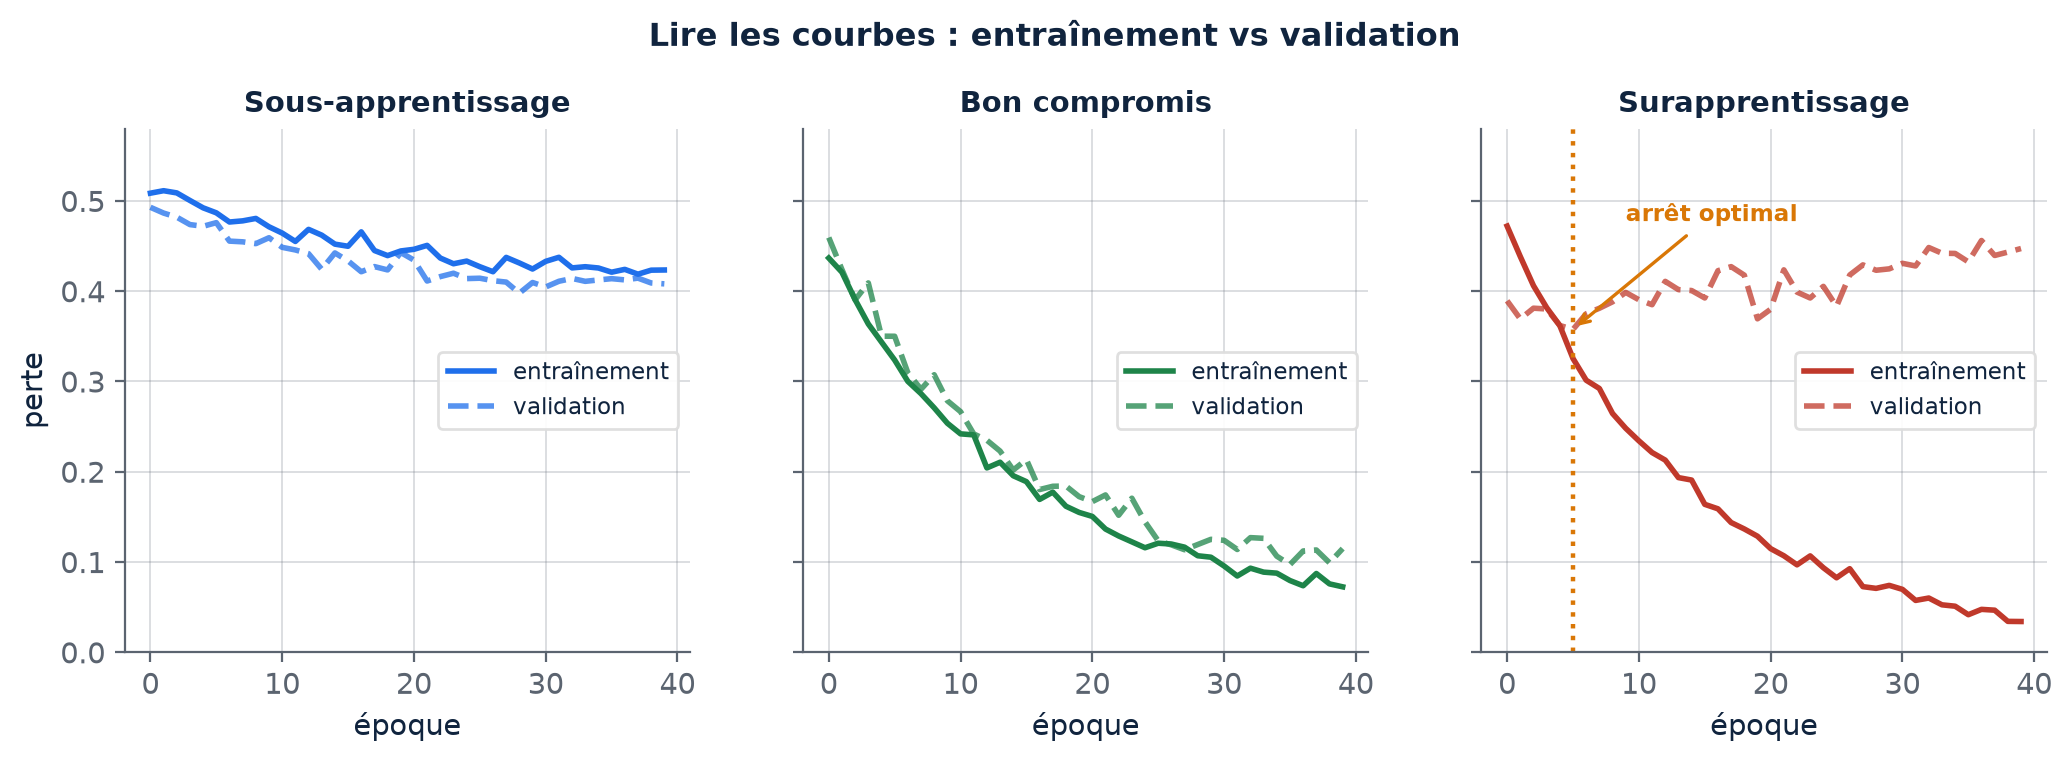
\includegraphics[width=\textwidth]{i01_courbes_apprentissage.png}
\end{column}
\begin{column}{0.46\textwidth}
\begin{itemize}
  \item On trace à chaque époque la perte d'\textbf{entraînement} et celle de
  \textbf{validation}.
  \item Ces deux courbes, comparées, disent tout : le modèle apprend-il,
  ou mémorise-t-il ?
  \item La courbe de validation est la seule qui compte : c'est elle qui
  mesure la capacité à généraliser.
\end{itemize}
\begin{kbox}[Règle d'or]
Ne jamais juger un modèle sur sa performance d'entraînement seule.
\end{kbox}
\end{column}
\end{columns}
\end{frame}

\begin{frame}{Lire les courbes : trois diagnostics}
\begin{columns}[t]
\begin{column}{0.32\textwidth}
\begin{wbox}[Sous-apprentissage]
Perte d'entraînement \emph{et} de validation hautes et plates.
Le modèle est trop simple, ou n'a pas assez appris.
\\[1mm]
{\small Ex. : $0{,}423$ (train) / $0{,}408$ (val).}
\end{wbox}
\end{column}
\begin{column}{0.32\textwidth}
\begin{ebox}[Bon compromis]
Les deux pertes baissent puis se stabilisent à des niveaux proches.
\\[1mm]
{\small Ex. : $0{,}072$ (train) / $0{,}115$ (val).}
\end{ebox}
\end{column}
\begin{column}{0.32\textwidth}
\begin{wbox}[Surapprentissage]
La perte d'entraînement continue de chuter, celle de validation remonte.
\\[1mm]
{\small Ex. : $0{,}034$ (train) / $0{,}447$ (val).}
\end{wbox}
\end{column}
\end{columns}
\vspace{1mm}
\begin{kbox}[Le diagnostic est visuel avant d'être chiffré]
Un écart qui se creuse entre les deux courbes = le réseau apprend du bruit
propre au jeu d'entraînement plutôt que le vrai motif.
\end{kbox}
\end{frame}

\begin{frame}{Le surapprentissage : reconnaître et anticiper}
\begin{columns}[t]
\begin{column}{0.52\textwidth}
\begin{itemize}
  \item \textbf{Symptôme} : l'écart train/validation se creuse à partir d'une
  certaine époque.
  \item \textbf{Ce n'est pas un échec} : c'est la frontière naturelle entre
  apprendre et mémoriser.
  \item \textbf{Remède} : arrêter au bon moment, ou régulariser (partie b).
\end{itemize}
\begin{kbox}[Le minimum utile]
La meilleure validation se lit à l'époque où sa courbe est la plus basse,
\emph{avant} qu'elle ne remonte.
\end{kbox}
\end{column}
\begin{column}{0.46\textwidth}
\begin{ebox}[Arrêt optimal : exemple]
Dans les courbes étudiées, la perte de validation atteint son minimum à
l'\textbf{époque 5}. Au-delà, elle remonte : le modèle surapprend.
\end{ebox}
\begin{wbox}[Pourquoi cela arrive ici]
Un petit jeu de données, un modèle à forte capacité et un grand nombre
d'époques : les trois ingrédients du surapprentissage réunis.
\end{wbox}
\end{column}
\end{columns}
\end{frame}

\begin{frame}[fragile]{Une boucle d'entraînement PyTorch minimale}
\begin{columns}[t]
\begin{column}{0.60\textwidth}
\begin{codebox}[Entraîner sur un jeu avec DataLoader]
\begin{lstlisting}
import torch
from torch.utils.data import DataLoader

train_loader = DataLoader(dataset, batch_size=64,
                          shuffle=True)
model = CNN()
loss_fn  = torch.nn.CrossEntropyLoss()
opt = torch.optim.Adam(model.parameters(), lr=1e-3)

for epoch in range(10):
    model.train()
    for x, y in train_loader:
        y_hat = model(x)
        loss  = loss_fn(y_hat, y)
        opt.zero_grad()   # 1. gradients a zero
        loss.backward()   # 2. retropropagation
        opt.step()        # 3. mise a jour des poids
\end{lstlisting}
\end{codebox}
\end{column}
\begin{column}{0.38\textwidth}
\begin{itemize}
  \item \py{shuffle=True} mélange les exemples à chaque époque.
  \item \py{model.train()} met le modèle en mode entraînement (dropout et BN
  actifs).
  \item Les trois lignes du bas sont \emph{indissociables} et dans cet ordre.
\end{itemize}
\begin{kbox}[Le strict minimum]
C'est tout le cœur de l'entraînement : dix lignes bien rangées.
\end{kbox}
\end{column}
\end{columns}
\end{frame}
